\chapter{Timepix 2}
% v podstatě technická dokumentace Timepix 2, plus konkretni pozadavky pro provoz
\label{kap:3}

V předchozí kapitole, kapitole \ref{kap:2}, byly popsány obecné vlastnosti detektoru a základní principy detekce ionizujícího záření. V této kapitole bude detailněji popsán konkrétní detektor, detektor Timepix 2 \cite{tpx2_manual}. Timepix 2 patří do rodiny detektorů Timepix. Prvním z rodiny detektorů byl detektor Timepix \cite{Llopart}, následně to popořadě byly detektory Timepix 3 \cite{Timepix3}, Timepix 2 \cite{tpx2_manual}, \cite{Timepix2} a nejnovějším detektorem je Timepix 4 \cite{Timepix4}. Detektor Timepix 2 je zobrazen na obrázku \ref{fig:Timepix2}.

\begin{figure}[h!]
	\centering
	\captionsetup{justification=centering}
	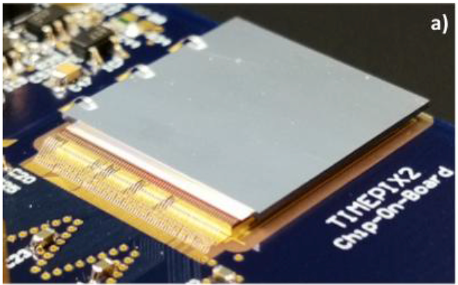
\includegraphics[scale=0.55]{Timepix2.png}
	\caption{Detektor Timepix 2 \cite{Timepix2}} 
	\label{fig:Timepix2}
\end{figure}	
\section{Technická specifikace} %napáječky, kom. rozhraní, prikazy atd.., VN, hodiny pro měření, I/O piny
Timepix 2 je rozdělen do 256 x 256 pixelů. Rozteč mezi jednotlivými pixely je 55 $\mu$$m$. Celkově pak Timepix 2 má rozměry 16.6 x 14.14 mm. Detektor byl vyvinut pod záštitou CERN Medpipix Collaboration \cite{Medpix}. Vyčítací část detektoru tvoří ASCI chip navržen ve 130 nm CMOS technologii. Samotná výroba ASIC je zajišťována jedním z předních výrobců chipů, firmou TSMC \cite{TSMC} na Taiwanu. Všechny technické informace, nebude-li uvedeno jinak jsou čerpány z manuálu k detektoru Timepix 2 \cite{tpx2_manual}.
\subsection{Napájení}	
Timepix 2 ke své činnosti potřebuj celkem 3 napájení viz. tabulka \ref{tab:tpx2_napajeni}. Napájení VDD a VDDA slouží k napájení jádra Timepix 2, napájení VDDIO pak k napájení vstupních výstupních bran. Pokud chceme z Timepix 2 vyčíst CHIP ID, musíme na pin VDD33 aplikovat napájecí napětí 2.5 V. Při normální činnosti detektoru, je požadováno napětí 1.2 V.  
\begin{table}[h!]
	\centering
	\begin{tabular}{ |P{3cm}||P{5cm}|  }
		\hline
		\multicolumn{2}{|c|}{Napájecí úrovně Timepix 2} \\
		\hline
		Název pinu& Hodnota napájecího napětí [V] \\ \hline \hline 
		VDDIO & 2.5 \\ \hline		
		VDD & 1.2 \\ \hline 		 
		VDDA & 1.2 \\ \hline
		VDD33 & 2.5 (1.2)\\ \hline
	\end{tabular}
	\caption{Napájecí úrovně Timepix 2}
	\label{tab:tpx2_napajeni}
\end{table}

\subsection{Rozhraní pro připojení Timepix 2 k desce plošných spojů}	% wirebondy
Připojení Timepix 2 k desce plošných spojů je nejčastěji realizováno pomocí technologie \textit{wire bonding}. Timepix 2 má celkem 152 pinů pro přichycení wire bondů. Rozložení pinů je zobrazeno na obrázku \ref{fig:tpx2_floorplan} ve spodní části. Rozteč mezi jednotlivými plošky je 108 $\mu$m.
\begin{figure}[h!]
	\centering
	\captionsetup{justification=centering}
	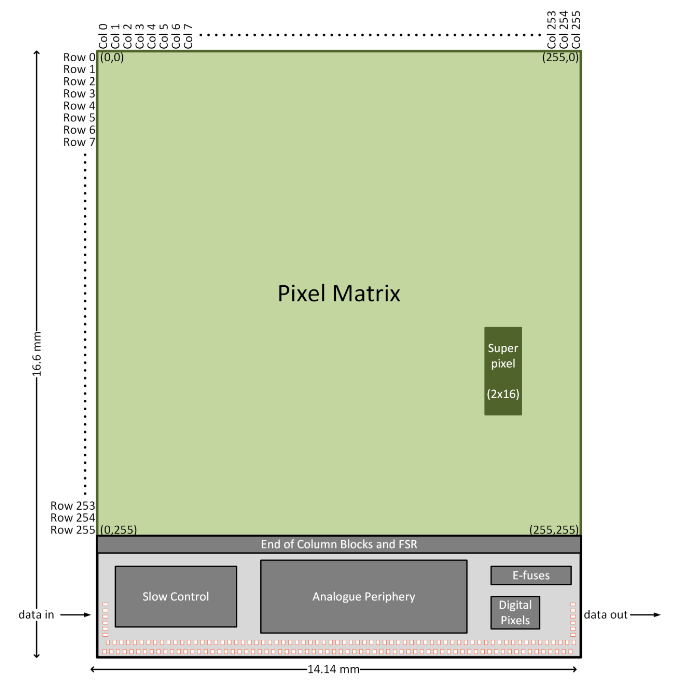
\includegraphics[scale=0.80]{tpx2_floorplan.png}
	\caption{Rozložení detektoru Timepix 2 \cite{tpx2_manual}} 
	\label{fig:tpx2_floorplan}
\end{figure}	

Dalším možným způsobem připojení Timepix 2 k desce plošných spojů je pomocí technologie zvané TSV. Respektive pomocí této technologie je možné signály vyvést ze zadní strany Timepix 2 k pájecím ploškám. Vznikne tím tak uspořádání, známe z technologie výroby pouzder BGA elektronických součástek. 
\par Běžnější způsob připojení Timepix 2 k desce plošných spojů je pomocí wire bondů. Použití wire bondů i technologie BGA je možné vidět na obrázku \ref{fig:bga}. Výhodou oproti technologii wire bondů je lepší praktické zacházení, díky absenci tenkých wire bondů, které jsou velmi náchylné na mechanické poškození. Další výhodou je poté technologicky méně náročné připojení detektoru. Avšak nevýhodou této technologie je vystavení chipu vysoké teplotě při pájení.
\begin{figure}[h!]
	\centering
	\captionsetup{justification=centering}
	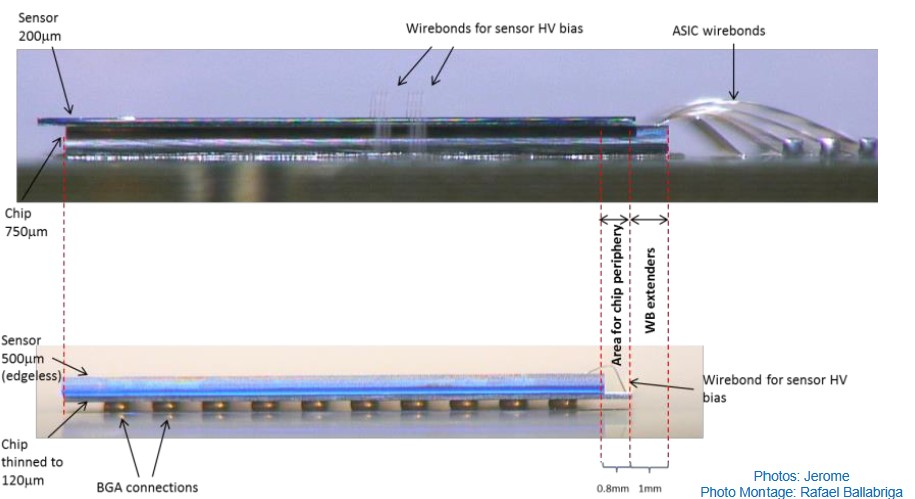
\includegraphics[scale=0.55]{bga.jpg}
	\caption{Připojení detektoru Timepix 2 k desce plošných spojů \cite{TSV}} 
	\label{fig:bga}
\end{figure}	

\section{Komunikační rozhraní}
\subsection{Datové rozhraní} %plus rychlosti komunikace 
% TODO pozor zminit i paraelni branu
Timepix 2 umožňuje komunikaci po paraelním nebo sériovém datovém kanálu. Pro komunikaci přes paraelní bránu je možno využít 32 paraelních vodičů. Paraelní brána se  
Veškerá seriová komunikace probíhá po diferenciálních datových párech. Konkrétně se jedná o specifikaci SLVS \cite{SLVS}. Napěťové úrovně této specifikace lze najít na obrázku \ref{fig:SLVS_LVDS}.
\begin{figure}[h!]
	\centering
	\captionsetup{justification=centering}
	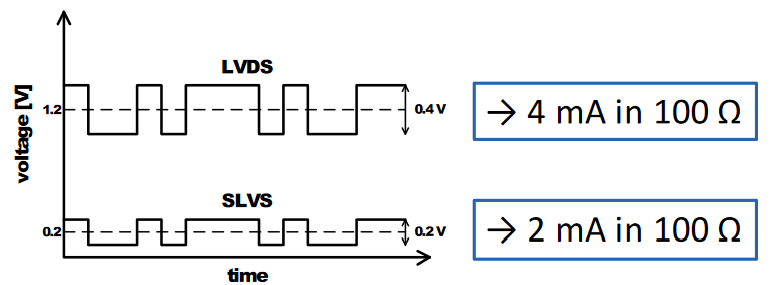
\includegraphics[scale=0.55]{SLVS_LVDS.png}
	\caption{SLVS specifikace \cite{SLVS}} 
	\label{fig:SLVS_LVDS}
\end{figure}	

%TODO popis signalu SPI pro TPX2 a casovani. Zminit i pakety SET/GET a jejich strukturu? 

\subsection{Vstupní, výstupní brána}

%TODO signaly potrebne pro komunikaci, ale pak i dac out atd.. 

% TODO zminit potrebne HV

\section{Analogová část}


\section{Digitální část}
%TODO mody timepix 2
 

